% Lab 3 Report - Full Subtractor Implementation
\documentclass[a4paper,12pt]{article}
\usepackage{graphicx}
\usepackage{listings}
\usepackage{hyperref}
\usepackage{geometry}
\usepackage{xcolor}
\usepackage{amsmath}
\geometry{left=1in, right=1in, top=1in, bottom=1in}

\lstset{
    frame=single,
    numbers=left,
    numberstyle=\tiny,
    basicstyle=\ttfamily\small,
    keywordstyle=\color{blue},
    commentstyle=\color{cyan},
    stringstyle=\color{red},
    breaklines=true,
    backgroundcolor=\color{gray!10}
}

\title{Lab Report\\ CSE4010 Computer Architecture}
\author{}
\date{}

\begin{document}

\maketitle

\noindent \textbf{Name:} \underline{Zachary A. Hampton\hspace{5cm}} \hfill \textbf{Score:} \underline{\hspace{2cm}/10} \\
\textbf{Student ID:} \underline{008339494\hspace{6cm}} \hfill \textbf{Due:} \underline{03-02-2025} \\
\textbf{Lab:} \underline{Lab 3 - Full Adder and Full Subtractor Implementation\hspace{6cm}}

\section*{Report}
\begin{itemize}
    \item How can addition and subtraction of large numbers be performed by computers if they are only aware of numbers 0 and 1?
    \begin{itemize}
        \item Computers perform arithmetic operations on large numbers by breaking them down into binary digits and processing them one bit at a time. For multi-digit numbers:
        \begin{itemize}
            \item Addition is performed using full adders in cascade, where each full adder processes one bit position and handles the carry from the previous stage
            \item Subtraction is similarly performed using full subtractors in cascade, where each subtractor handles one bit position and processes the borrow from the previous stage
            \item The carry/borrow propagation between stages allows for handling numbers of any size
        \end{itemize}
        \item This binary arithmetic is implemented using combinational circuits that:
        \begin{itemize}
            \item Process bits from least significant to most significant position
            \item Use carry/borrow propagation for managing digit transitions
            \item Can be extended to any number of bits by cascading multiple stages
        \end{itemize}
    \end{itemize}
\end{itemize}

\section*{Source Code}
\subsection*{fullAdder.v}
\begin{lstlisting}[language=Verilog]
/*
 * File: fullAdder.v
 * Description: Implements a 1-bit full adder using half adders
 * A full adder adds three bits (A, B, and carry-in) and produces sum and carry-out
 * A full adder is built from two half adders and an OR gate; 
 * The first half adder adds A and B and produces a sum and a carry
 * The second half adder adds the carry from the first half adder to the carry-in
 * The OR gate adds the carries from the two half adders to produce the final carry-out
 */

// Half Adder Module - Adds two bits and produces sum and carry
module halfAdder(op1, op2, sum, carry);

    // Inputs - two 1-bit operands
    input op1, op2;
    // Outputs - sum and carry bits
    output sum, carry;
    
    // XOR operation - sum is 1 if either op1 or op2 is 1, but not both
    assign sum = op1 ^ op2; // ^ is the xor operator
    // AND operation - carry is 1 only if both op1 and op2 are 1
    assign carry = op1 & op2; // & is the and operator
    
endmodule

// Full Adder Module - Adds three bits (A, B, carry-in) and produces sum and carry-out
module fullAdder(A, B, Cin, sum, Cout);

    // Input ports
    input A, B, Cin;  // A and B are the bits to add, carryIn is the carry from previous addition
    // Output ports
    output sum, Cout; // sum is the result bit, carryOut propagates to next addition
    
    // Internal connections - wires to connect the half adders
    wire c;  // Sum output from first half adder
    wire d;  // Carry output from first half adder
    wire e;  // Sum output from second half adder
    wire f;  // Carry output from second half adder
    
    // First half adder - adds A and B
    halfAdder u1(A, B, c, d);
    // Second half adder - adds carryIn and the sum from first half adder
    halfAdder u2(Cin, c, e, f);
    
    // Final carry out is OR of both half adder carries
    assign Cout = f | d;  // | is the OR operator
    // Final sum is the sum output from second half adder
    assign sum = e;
    
endmodule
\end{lstlisting}

\subsection*{fullAdder\_tb.v}
\begin{lstlisting}[language=Verilog]
/*
 * File: fullAdder_tb.v
 * Description: Testbench for the 1-bit full adder
 * Tests all possible input combinations (0-7) for A, B, carryIn
 * The testbench uses a loop to iterate through all possible input combinations
 * It displays the results of each test case
 */
 
// Define timescale for simulation: 1 nanosecond time unit, 1 nanosecond precision
`timescale 1 ns / 1 ns
// Include the module to be tested
`include "fullAdder.v"

// Testbench module - no external ports
module fullAdder_tb;

// Test inputs - declared as registers since they will be driven
reg A, B, Cin;
// Test outputs - declared as wires since they will be monitored
wire sum, Cout;

// Instantiate the Unit Under Test (UUT) - connect to test signals
fullAdder uut(A, B, Cin, sum, Cout);

// Test sequence
initial begin
    // Generate VCD file for waveform viewing
    $dumpfile("fullAdder_tb.vcd");
    // Dump variables from the testbench (0 means all variables)
    $dumpvars(0, fullAdder_tb);
    
    // Test case 0: A=0, B=0, Cin=0
    {A, B, Cin} = 3'd0; #20;
    // Test case 1: A=0, B=0, Cin=1
    {A, B, Cin} = 3'd1; #20;
    // Test case 2: A=0, B=1, Cin=0
    {A, B, Cin} = 3'd2; #20;
    // Test case 3: A=0, B=1, Cin=1
    {A, B, Cin} = 3'd3; #20;
    // Test case 4: A=1, B=0, Cin=0
    {A, B, Cin} = 3'd4; #20;
    // Test case 5: A=1, B=0, Cin=1
    {A, B, Cin} = 3'd5; #20;
    // Test case 6: A=1, B=1, Cin=0
    {A, B, Cin} = 3'd6; #20;
    // Test case 7: A=1, B=1, Cin=1
    {A, B, Cin} = 3'd7; #20;
    // Display a message to indicate completion of test cases
    $display("Finished additions!");
    
end

endmodule
\end{lstlisting}

\subsection*{fullSubtractor.v}
\begin{lstlisting}[language=Verilog]
/*
 * File: fullSubtractor.v
 * Description: Implements a 1-bit full subtractor using half subtractors
 * A full subtractor subtracts three bits (A, B, and borrow-in) and produces difference and borrow-out
 * A full subtractor is built from two half subtractors and an OR gate; 
 * The first half subtractor subtracts B from A and produces a difference and a borrow
 * The second half subtractor subtracts the borrow-in from the difference of the first half subtractor
 * The OR gate combines the borrows from the two half subtractors to produce the final borrow-out
 */

// Half Subtractor Module - Subtracts one bit from another and produces difference and borrow
module halfSubtractor(op1, op2, diff, borrow);

    // Inputs - two 1-bit operands
    input op1, op2;
    // Outputs - difference and borrow bits
    output diff, borrow;

    // XOR operation - difference is 1 if op1 and op2 are different
    assign diff = op1 ^ op2;

    // AND operation with NOT on op2 - borrow is 1 if op1=1 and op2=0
    assign borrow = op1 & !op2;

endmodule

// Full Subtractor Module - Subtracts three bits (A, B, borrow-in) and produces difference and borrow-out
module fullSubtractor(A, B, Bin, diff, Bout);

    // Input ports
    input A, B, Bin;  // A is minuend, B is subtrahend, Bin is borrow-in from previous subtraction
    // Output ports
    output diff, Bout; // diff is the difference bit, Bout propagates borrow to next subtraction
    
    // Internal connections - wires to connect the half subtractors
    wire c;  // Difference output from first half subtractor
    wire d;  // Borrow output from first half subtractor
    wire e;  // Difference output from second half subtractor (unused)
    wire f;  // Borrow output from second half subtractor

    // First half subtractor - subtracts B from A
    halfSubtractor u1(A, B, c, d);

    // Second half subtractor - subtracts Bin from the result of first half subtractor
    halfSubtractor u2(c, Bin, diff, f);

    // Final borrow out is OR of both half subtractor borrows
    assign Bout = f | d;  // | is the OR operator

endmodule
\end{lstlisting}

\subsection*{fullSubtractor\_tb.v}
\begin{lstlisting}[language=Verilog]
/*
 * File: fullSubtractor_tb.v
 * Description: Testbench for the 1-bit full subtractor
 * Tests all possible input combinations (0-7) for A, B, Bin
 * The testbench uses a loop to iterate through all possible input combinations
 * It displays the results of each test case
 */
 
// Define timescale for simulation: 1 nanosecond time unit, 1 nanosecond precision
`timescale 1 ns / 1 ns
// Include the module to be tested
`include "fullSubtractor.v"

// Testbench module - no external ports
module fullSubtractor_tb;

// Test inputs - declared as registers since they will be driven
reg A, B, Bin;
// Test outputs - declared as wires since they will be monitored
wire diff, Bout;

// Instantiate the Unit Under Test (UUT) - connect to test signals
fullSubtractor uut(A, B, Bin, diff, Bout);

// Test sequence
initial begin
    // Generate VCD file for waveform viewing
    $dumpfile("fullSubtractor_tb.vcd");
    // Dump variables from the testbench (0 means all variables)
    $dumpvars(0, fullSubtractor_tb);
    
    // Test case 0: A=0, B=0, Bin=0
    {A, B, Bin} = 3'd0; #20;
    // Test case 1: A=0, B=0, Bin=1
    {A, B, Bin} = 3'd1; #20;
    // Test case 2: A=0, B=1, Bin=0
    {A, B, Bin} = 3'd2; #20;
    // Test case 3: A=0, B=1, Bin=1
    {A, B, Bin} = 3'd3; #20;
    // Test case 4: A=1, B=0, Bin=0
    {A, B, Bin} = 3'd4; #20;
    // Test case 5: A=1, B=0, Bin=1
    {A, B, Bin} = 3'd5; #20;
    // Test case 6: A=1, B=1, Bin=0
    {A, B, Bin} = 3'd6; #20;
    // Test case 7: A=1, B=1, Bin=1
    {A, B, Bin} = 3'd7; #20;
    // Display a message to indicate completion of test cases
    $display("Finished subtractions!");
    
end

endmodule
\end{lstlisting}

\section*{Screenshots}
\subsection*{Part A - Full Adder Simulation}
\begin{figure}[h]
    \centering
    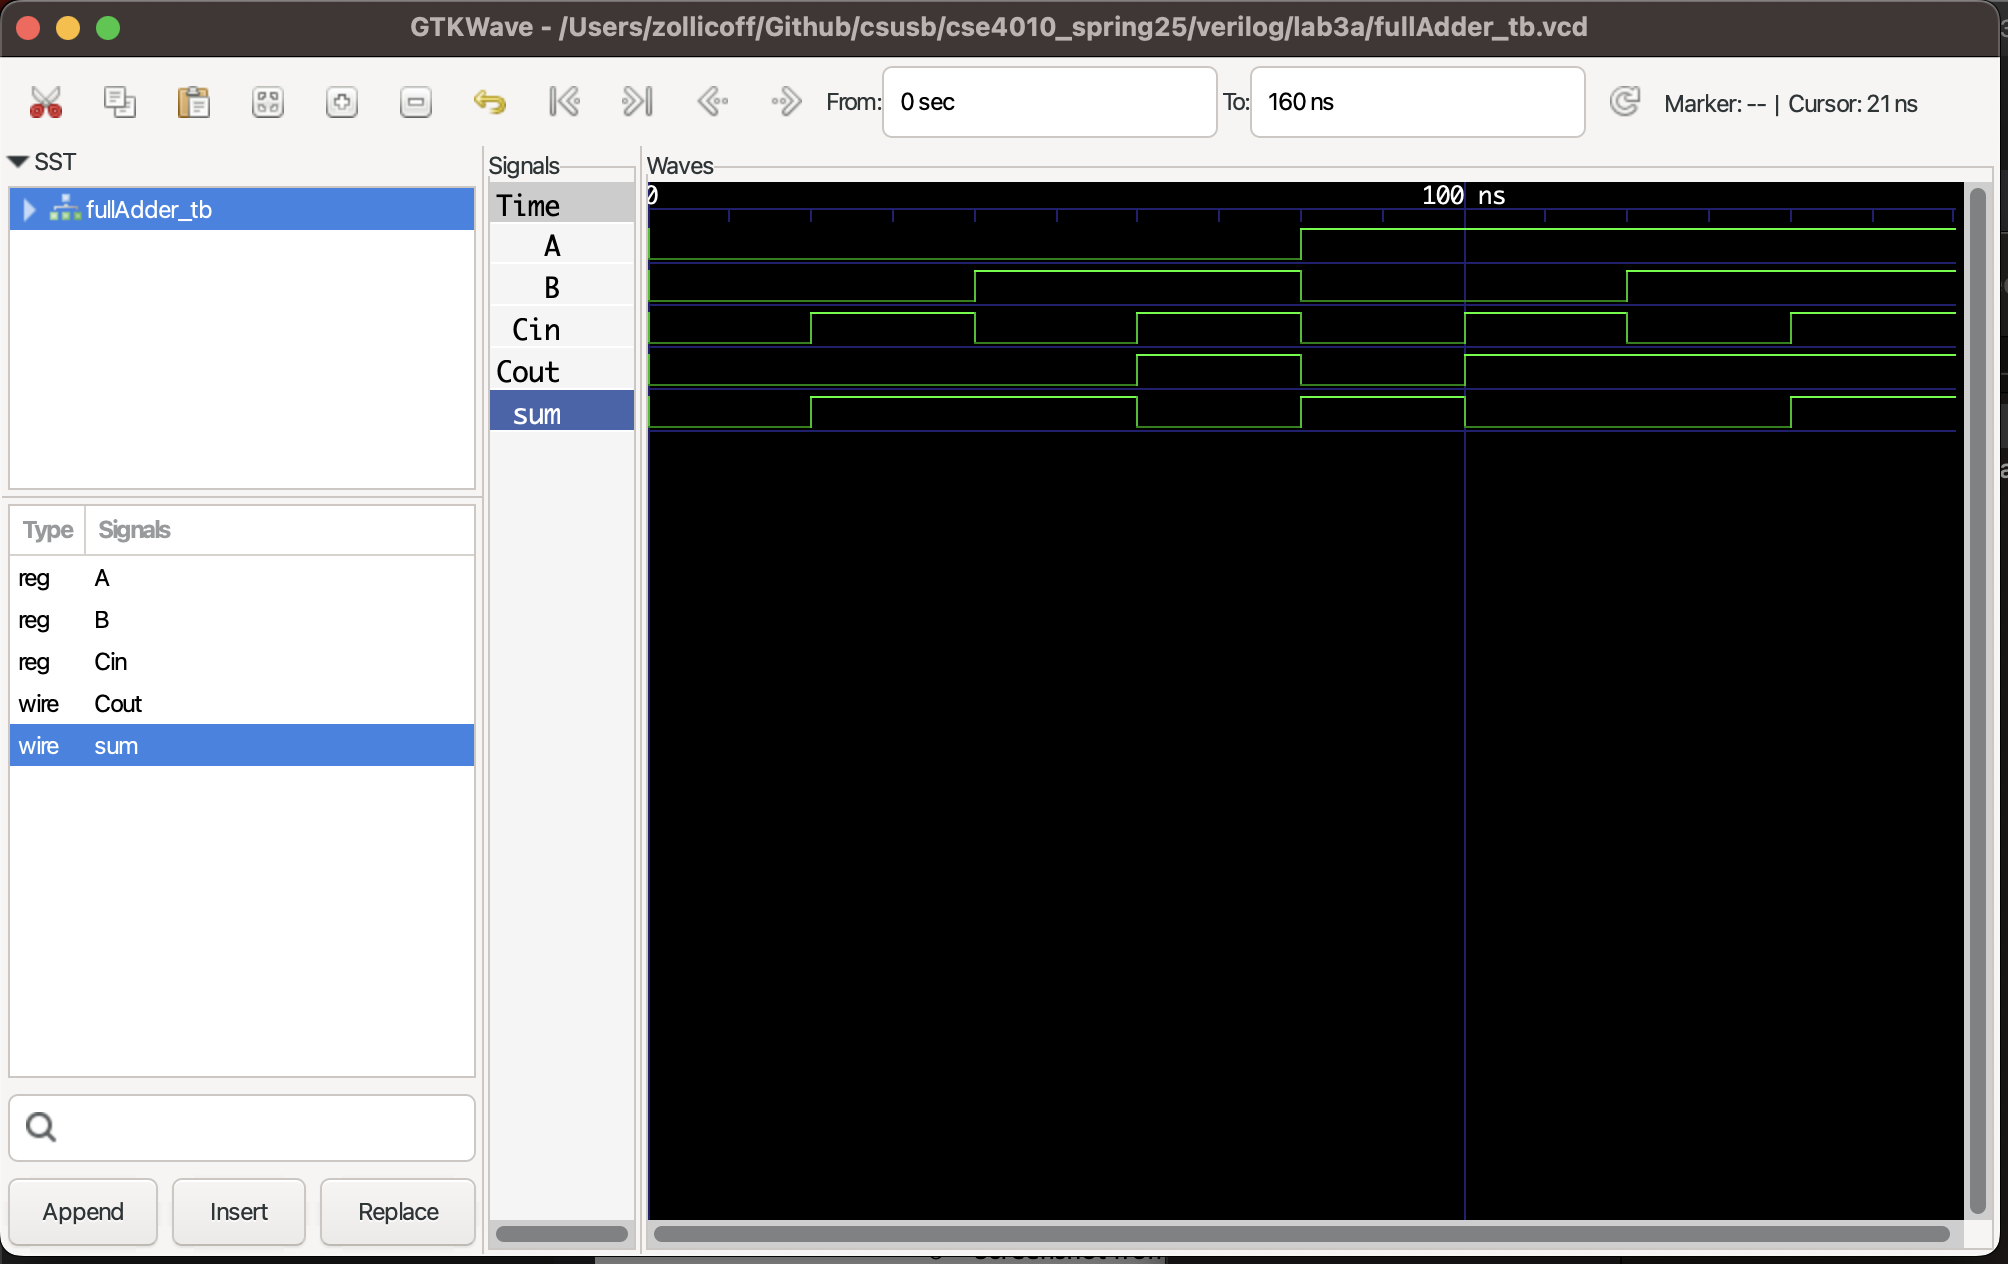
\includegraphics[width=\textwidth]{full_adder.png}
    \caption{Full Adder Simulation Waveform showing all test cases with inputs A, B, Cin and outputs sum, Cout}
\end{figure}

\subsection*{Part B - Full Subtractor Simulation}
\begin{figure}[h]
    \centering
    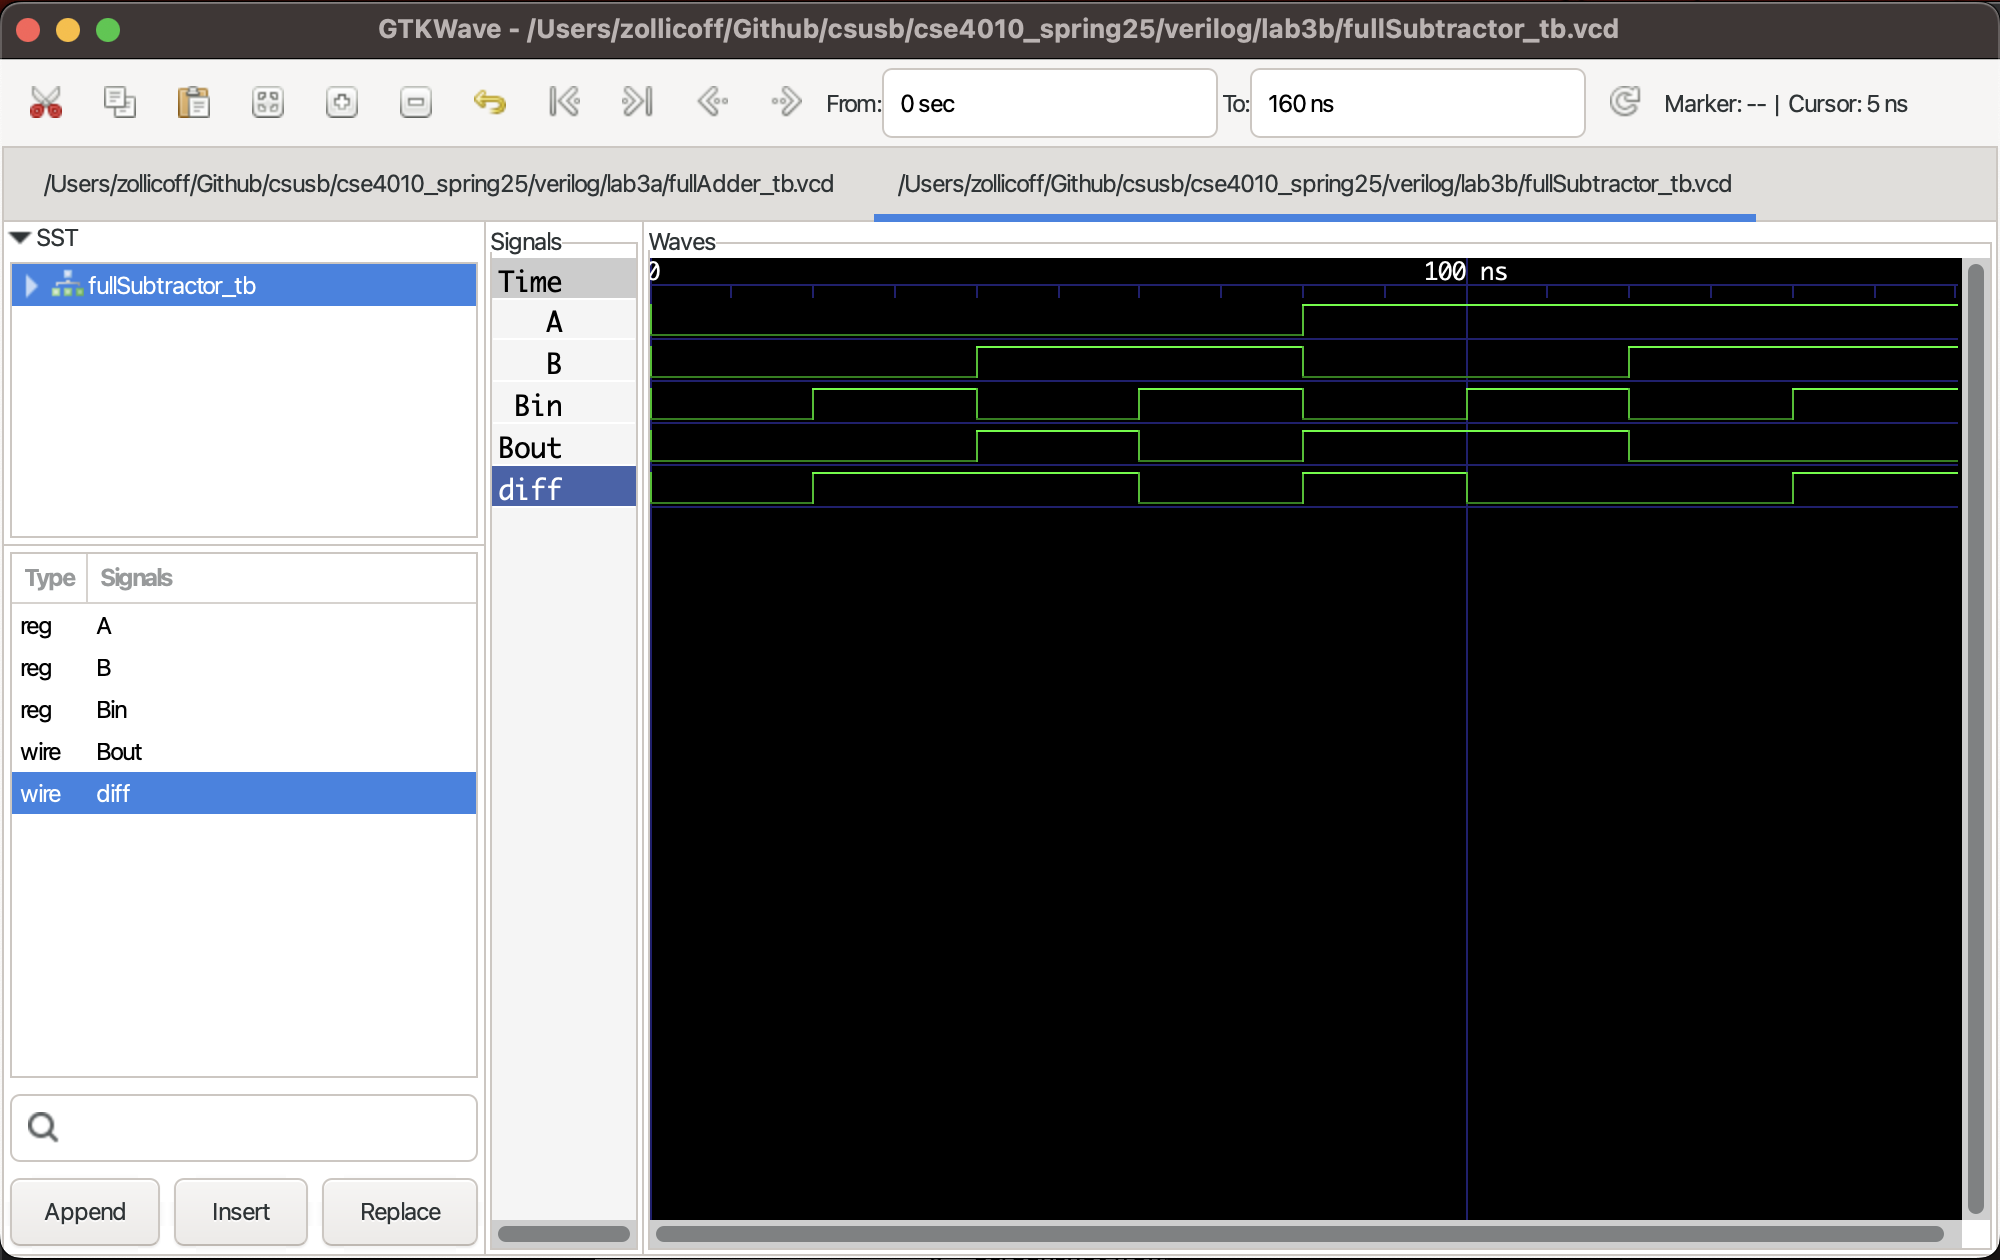
\includegraphics[width=\textwidth]{full_subtractor.png}
    \caption{Full Subtractor Simulation Waveform showing all test cases with inputs A, B, Bin and outputs diff, Bout}
\end{figure}

\end{document} 